% !TeX spellcheck = en_US
% !TeX encoding = UTF-8
\section{Umbrella Sampling\label{Sec:ES:US}}
Umbrella Sampling method was proposed by Torrie and Valleau in 1977,\cite{TorrieJComputP1977} and is still widely used nowadays.
Suppose we are studying a transition process between states such as conversion between two dominant conformations or a chemical reaction, and these two states are separated by a high barrier relative to $kT$. Therefore, the transition is a rare even. A schematic representation of the free energy landscape is shown in Fig.~\ref{Fig:ES:dual_harmonic}.
\begin{figure}[htbp]
	\centering
	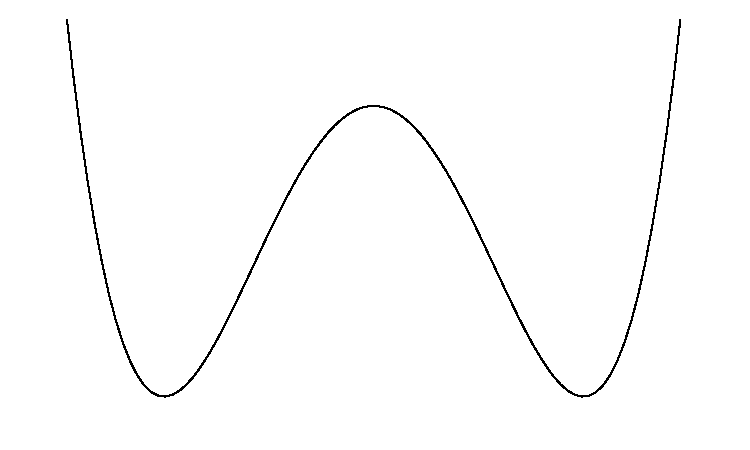
\includegraphics[width=0.6\textwidth]{figures/dual_harmonic.pdf}\\
	\caption{}\label{Fig:ES:dual_harmonic}
\end{figure}

Sometimes, we are interested in not only these two dominate states but also the states in between. Usually, we define a reaction coordinate $\xi$ and calculate the potential of mean force along this reaction coordinate from the ``reactant'' to the ``product''. However, if we run a simulation with the reaction coordinate initially set to the transition state or on the hill, the system will quickly roll back to the ``reactant'' or the ``product'' state in order to reduce the free energy. The consequence is that regions outside the ``reactant'' and ``product'' regions cannot be sampled sufficiently to yield accurate free energy profile in a brutal force simulation. In order to increase the sampling in these regions, we can modify the potential energy surface by introducing a series of biases as (usually harmonic) functions of $\xi$ to the system. Each biased simulation is called a \textit{window}. The strengths of the biases should be strong enough to maintain the system in the vicinity of where you are interested in, and also should be weak enough that the system can have significant overlap in two adjacent windows. After all the simulations, the whole region is well sampled and the free energy profile can be generated using Weighted Histogram Analysis Method or the Multistate Bennett Acceptance Ratio method (to be discussed in Section~\ref{Sec:FEM:WHAM} and~\ref{Sec:FEM:MBAR}).